\section{Experimental Setup}

\begin{figure}[H]
    \centering
    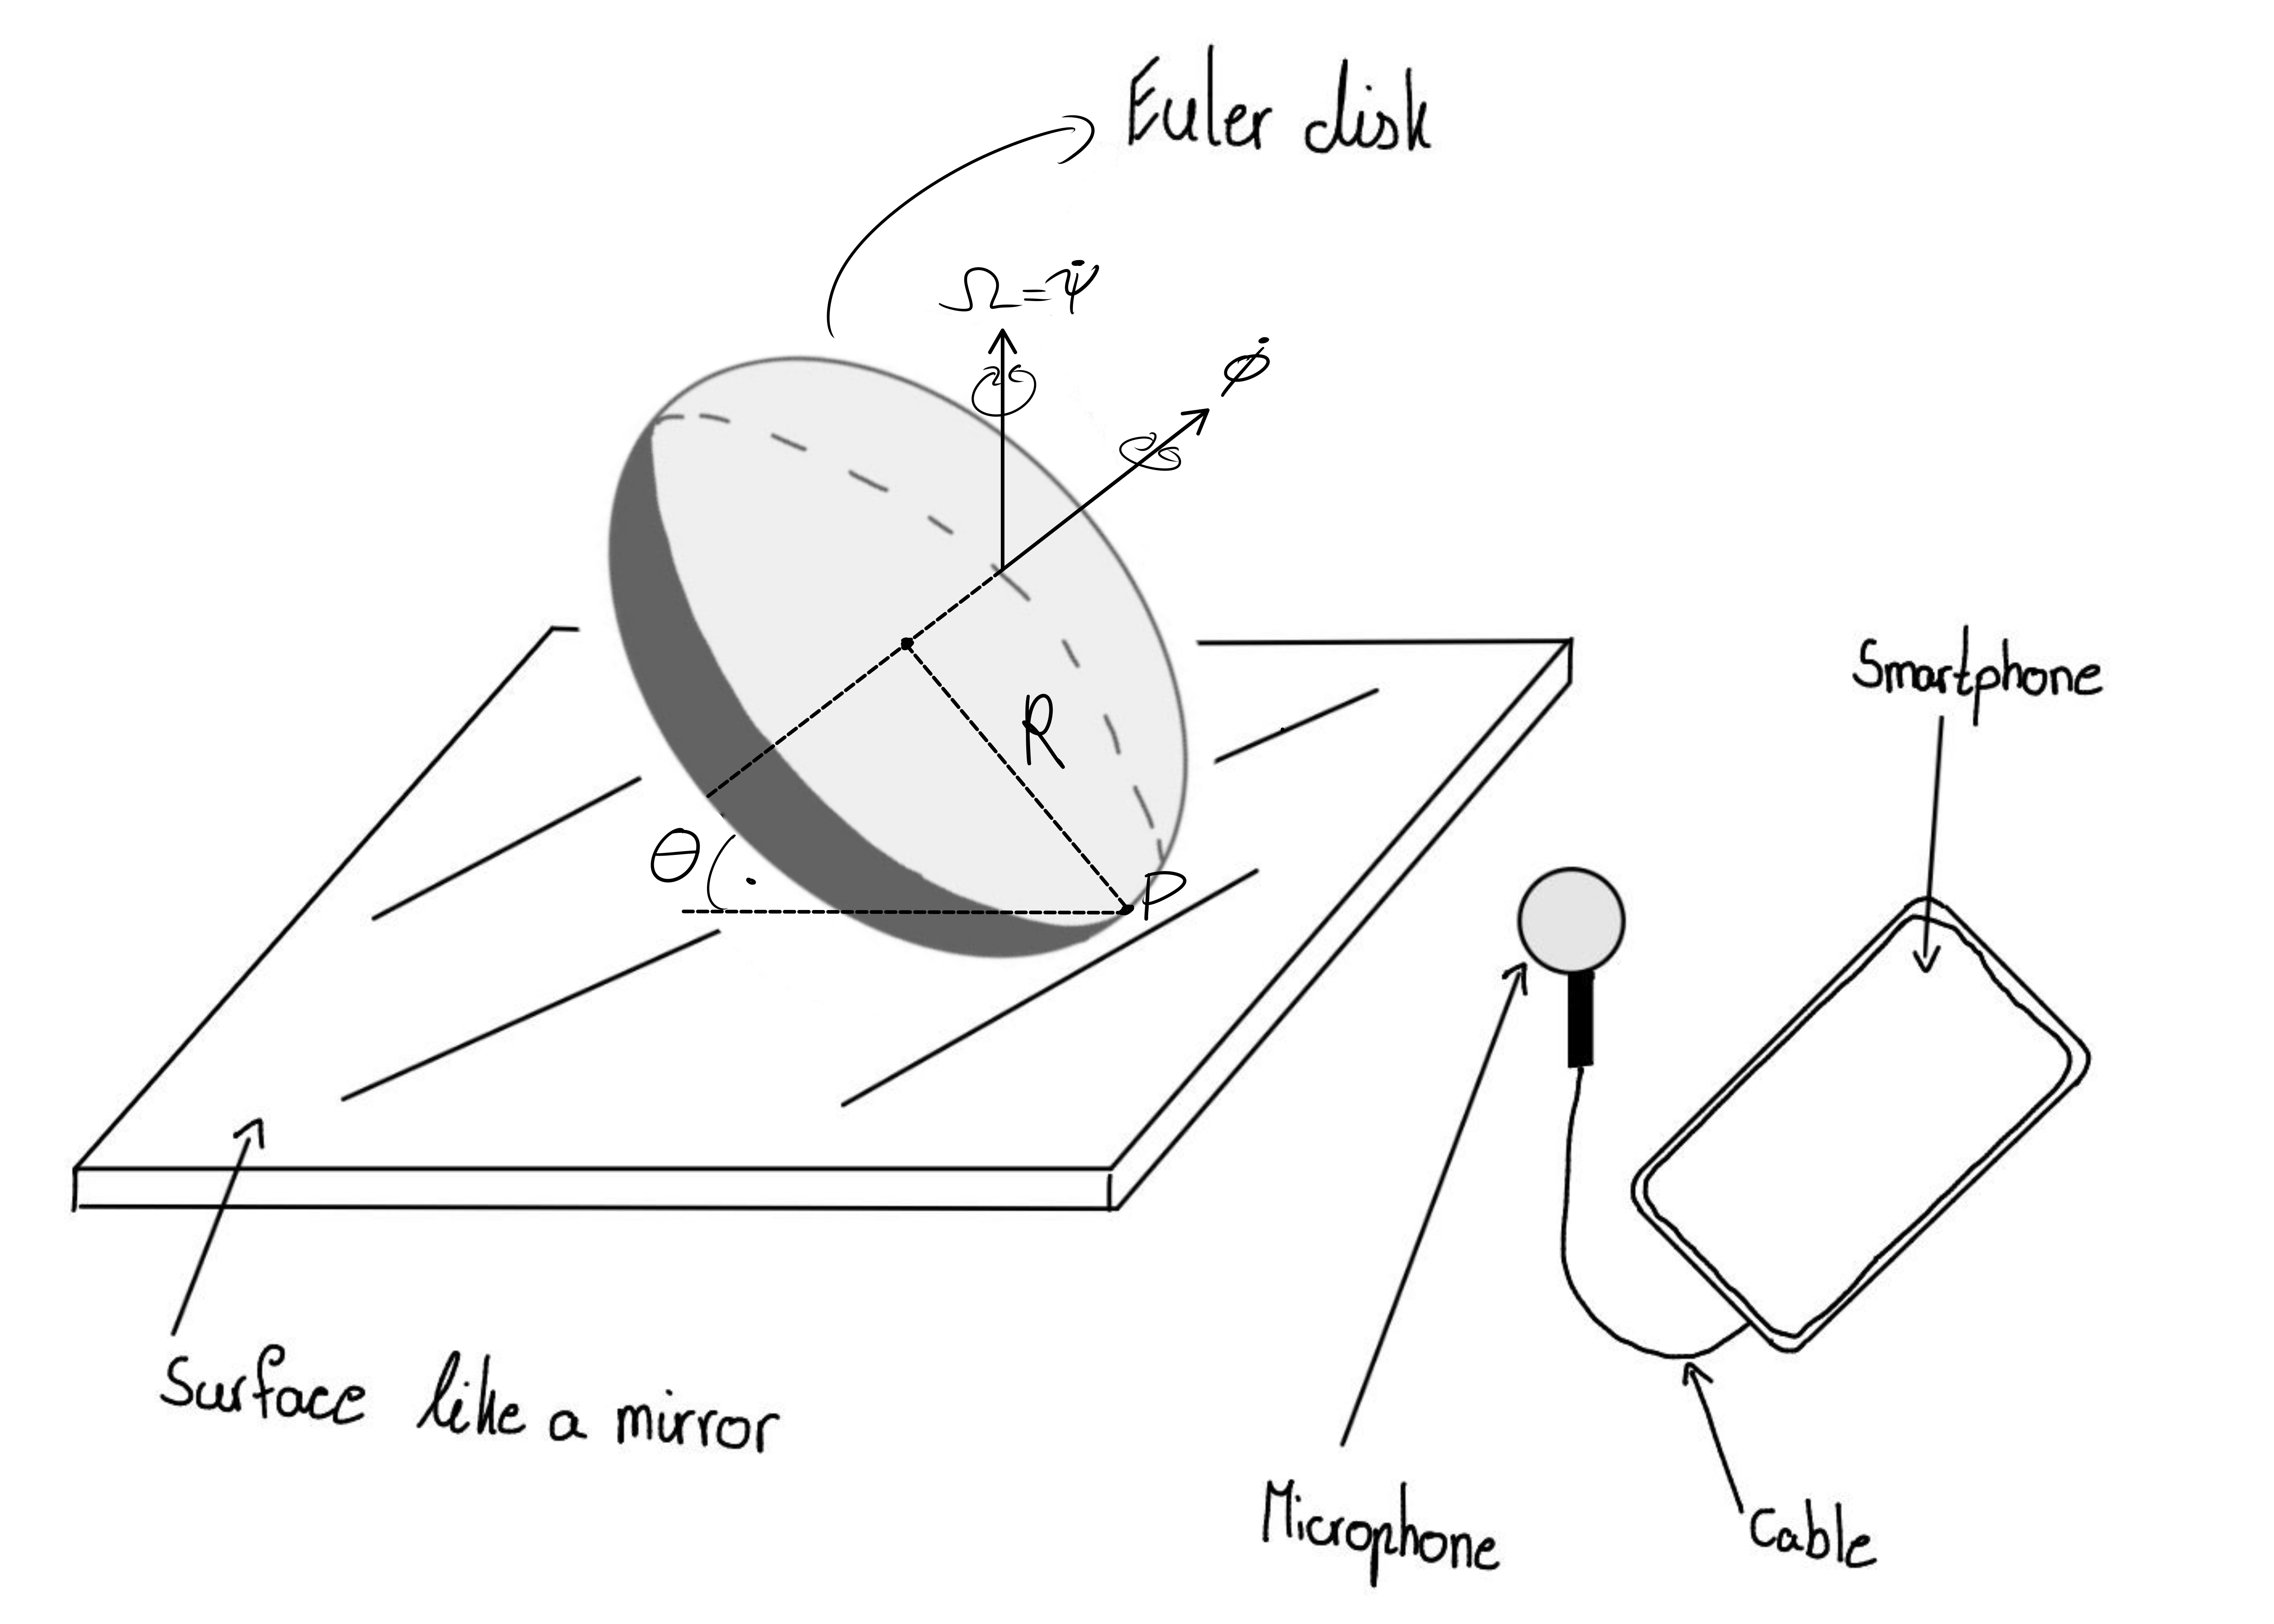
\includegraphics[width=0.7\textwidth]{figures/euler_disc_primitive_sketch.png}
    \caption{A primitive sketch of the outlines of the experimental setup showing the Euler disk, the surface and the relevant quantities: the radius of the Euler disc $R$, the contact point between the disc and the surface $P$, the precession rate $\Omega=\dot{\psi}$, the spin rate $\dot{\phi}$, and the tilt angle $\theta$. Furthermore, the measurement device, also the smartphone with a microphone is shown on the same sketch.}
    \label{fig:euler_disc_primitive_sketch}
\end{figure}

The main elements of the experimental setup consists of a rigid circular disk also known as the Euler's disk spun on a flat horizontal surface. The disk of radius $R$ is inclined at an angle $\theta$ with respect to the surface and makes contact at a single point $P$, which moves around the center of mass with precession frequency $\Omega$. As the disk evolves in time, both the inclination angle and the precession rate change continuously.

The Euler disk is set into motion using two pendulums. The use of two pendulums is intended to reduce the initial linear motion caused by the impact and to produce a more controlled rotational excitation. The disk spins on a thick, smooth stone layer placed on top of a table in order to provide a stable surface and reduce interfering vibrations from the table.

The motion of the disk is recorded using two smartphones. One phone will be placed above the disk to record its motion in the horizontal plane. A marked line on the disk will be used to track its radial motion during the experiment. A second phone will be placed approximately at the height of the disk where it touches the surface in order to record the angle between the disk and the surface. Strong lighting will be used to overexpose the bright background in the video, so that the disk appears as a dark object with high contrast. This setup is intended to simplify the later video analysis.

At the same time, the sound emitted by the disk will be recorded. The recorded audio data will be analyzed using Fourier-based spectral methods in order to extract the time-dependent dominant frequency $f(t)$. The video recordings will be analyzed separately to determine the radial motion and the tilt angle of the disk. This allows the results from the acoustic analysis and the video analysis to be compared with each other.

\begin{figure}[H]
    \centering
    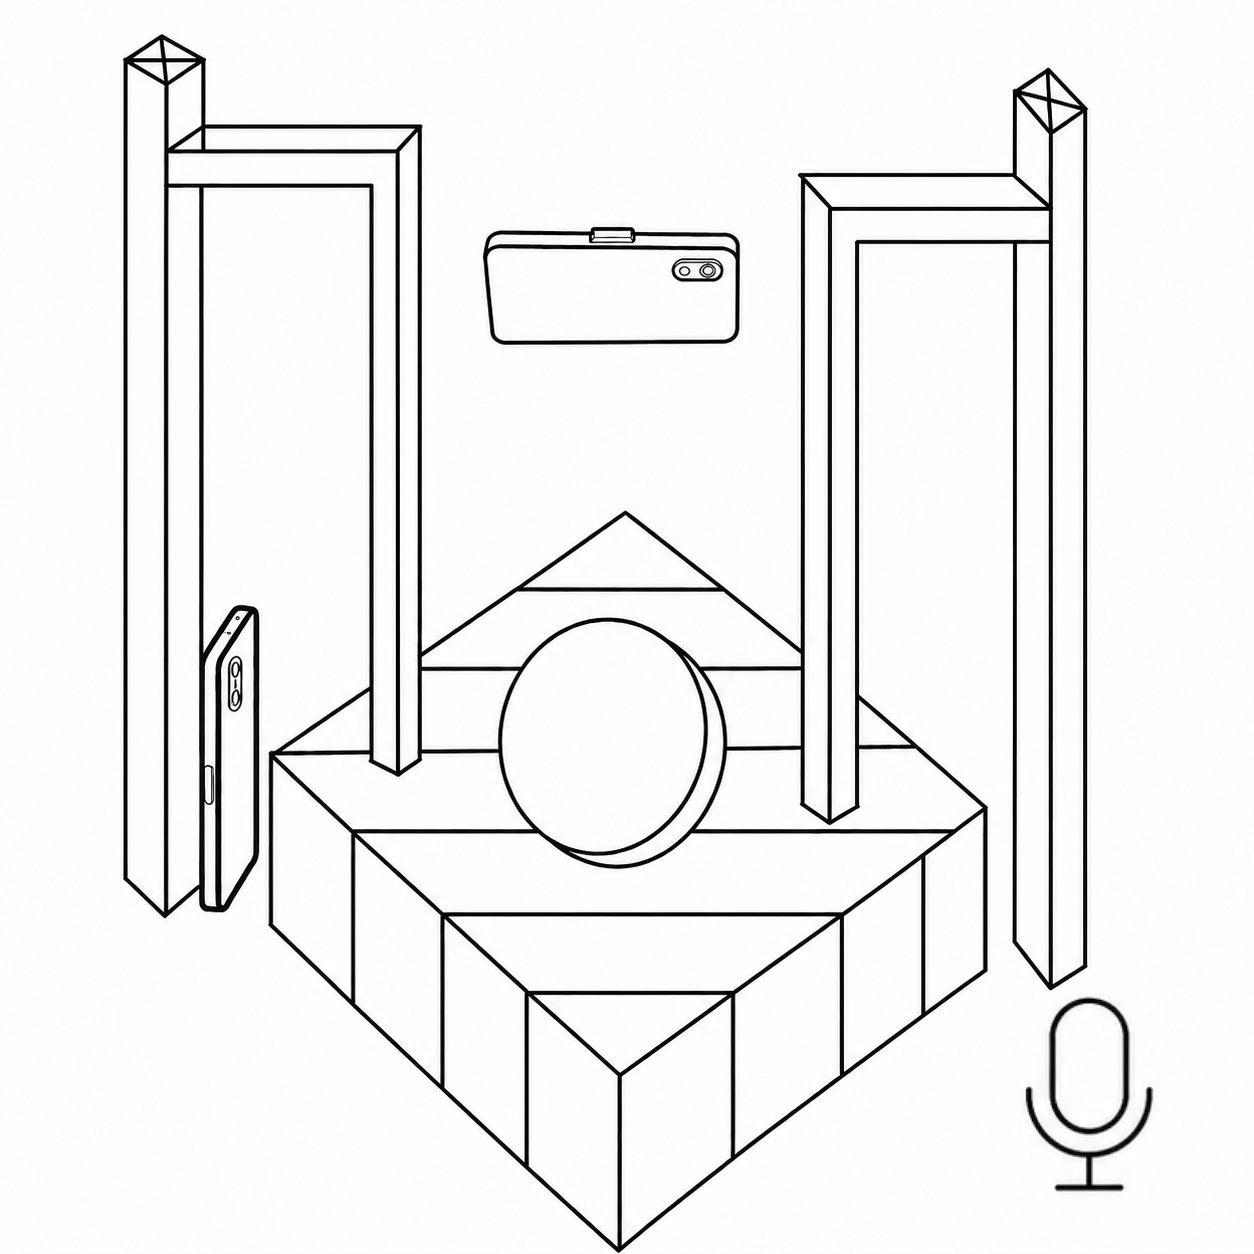
\includegraphics[width=0.5\textwidth]{figures/euler_disc_exact_sketch.png}
    \caption{The sketch of the exact setup including the surface, the Euler's disc, the two phones used for visual measurements and their positions as well as the audio recorder which can either be another phone or specialized device.}
    \label{fig:euler_disc_exact_sketch}
\end{figure}
